% --- INICIO DEL MÓDULO SINTETIZADO: 05_preguntas_o_x.tex ---

\subsection{Conformación de Pulso, Códigos de Línea y Modulación (6.o - 6.x)}

La alteración paramétrica del filtro interpolador $h$ y las Muestras por Símbolo ($Sps$) permite adaptar la señal a las restricciones del canal. En el límite teórico ($Sps=1$), la señal pierde su envolvente temporal, convirtiéndose en muestras aleatorias descorrelacionadas cuyo espectro es plano, equivalente a ruido blanco discreto (6.o). Al restaurar un $Sps=4$, se evaluaron diferentes geometrías de pulso. El uso de una rampa asimétrica o Diente de Sierra ($h=[0.25, 0.5, 0.75, 1]$) (6.p) genera transiciones abruptas que degradan la atenuación de los lóbulos laterales en la Densidad Espectral de Potencia (PSD), incrementando la interferencia de canal adyacente. Por otro lado, el formato RZ ($h=[1, 1, 0, 0]$) (6.q) retorna a cero a mitad del símbolo; esta compresión temporal duplica el consumo de ancho de banda ($2R_b$). En contraste, el código Manchester ($h=[1, 1, -1, -1]$) (6.r) fuerza una transición interna que equilibra el área de voltaje a cero. Esto elimina por completo el impulso ineficiente de Corriente Continua en $0\text{ Hz}$, demostrando la superioridad energética de los formatos bipolares balanceados frente a los unipolares (6.x).

Para trasladar la información a radiofrecuencia (paso-banda), se inyectaron arreglos senoidales (\texttt{np.sin}) en el filtro. Las modulaciones de amplitud como OOK y ASK (6.s, 6.u) desplazan el espectro, pero desperdician potencia al transmitir una portadora pura. Sin embargo, al mantener datos de entrada bipolares, se logra la modulación BPSK (6.t). En este esquema, los bits negativos invierten matemáticamente la senoide, generando saltos de fase de $180^\circ$ que suprimen la portadora central en la PSD, maximizando la eficiencia de transmisión.

Finalmente, para la mitigación de la Interferencia Intersimbólica (ISI), se implementaron pulsos tipo sinc (6.v) y filtros de Raíz de Coseno Alzado (6.w). El uso de la función \texttt{firdes.root\_raised\_cosine} demostró ser el esquema de mayor eficiencia espectral: sus oscilaciones temporales amortiguadas ("pulsos rizados") logran anular de forma absoluta los lóbulos laterales en la frecuencia, confinando la energía de la señal en un bloque libre de fugas espectrales.

% --- FIGURA DE SÍNTESIS (3 SUBFIGURAS CLAVE) ---
\begin{figure}[htbp]
\centering
\begin{subfigure}[b]{0.5\textwidth}
    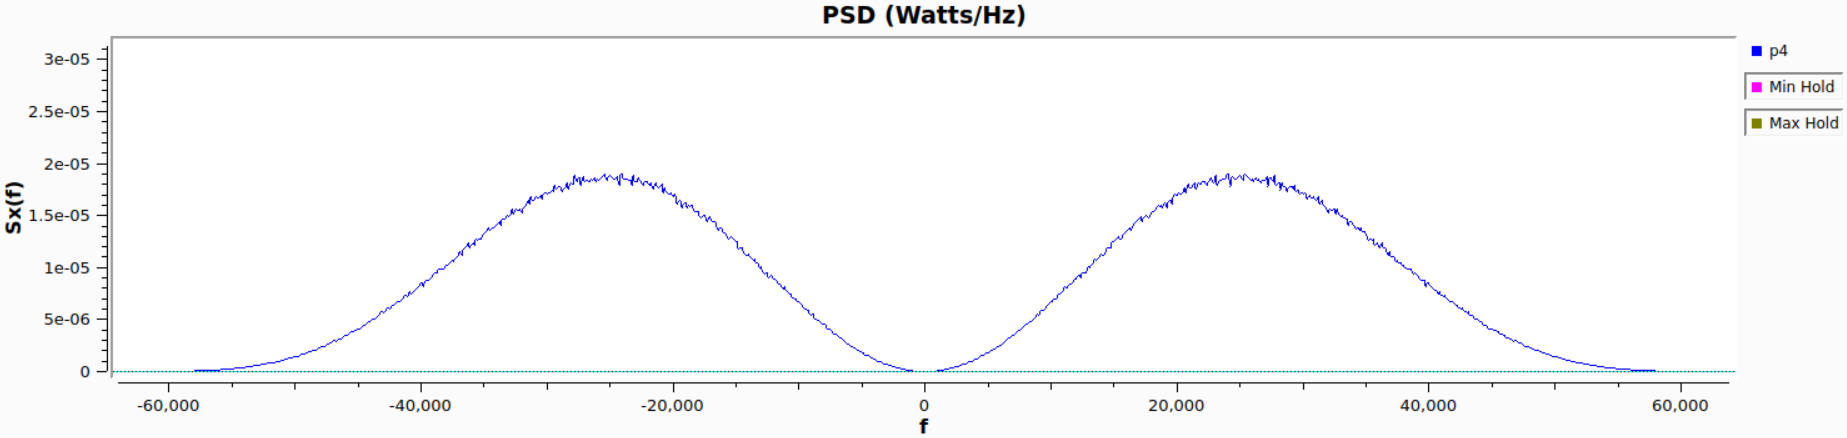
\includegraphics[width=\textwidth]{imagenes/captura_manchester.png} % Usa tu captura de la PSD de Manchester
    \caption{PSD Manchester: Eliminación de la componente DC.}
    \label{fig:sintesis_manchester}
\end{subfigure}
\hfill
\begin{subfigure}[b]{0.5\textwidth}
    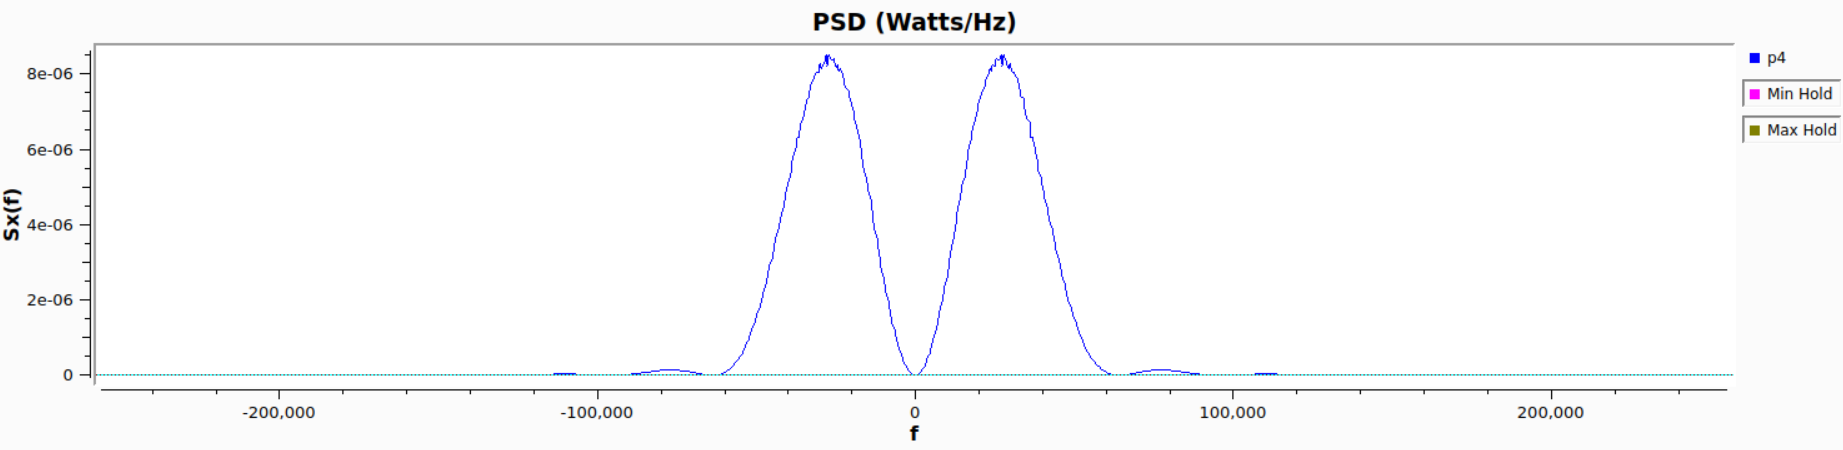
\includegraphics[width=\textwidth]{imagenes/captura_bpsk.png} % Usa tu captura del tiempo (osciloscopio) de BPSK
    \caption{BPSK (Tiempo): Saltos de fase de $180^\circ$.}
    \label{fig:sintesis_bpsk}
\end{subfigure}
\hfill
\begin{subfigure}[b]{0.5\textwidth}
    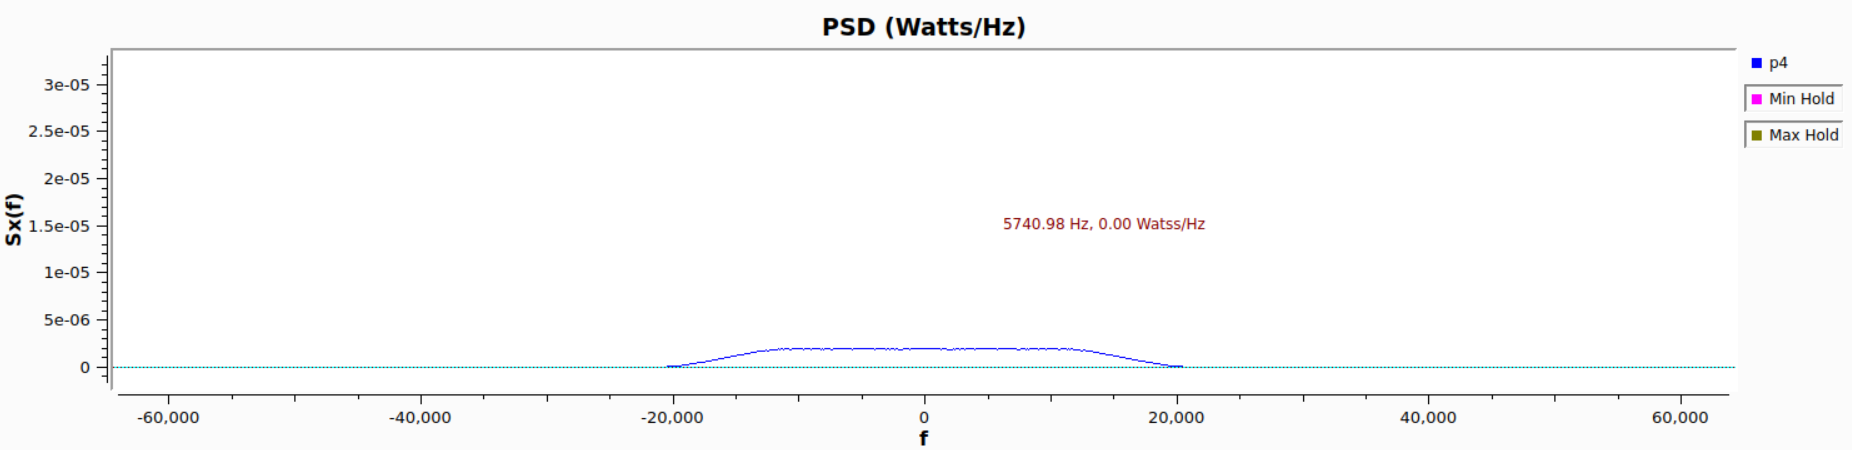
\includegraphics[width=\textwidth]{imagenes/captura_coseno.png} % Usa tu captura de la PSD del Coseno Alzado
    \caption{PSD Coseno Alzado: Supresión de lóbulos laterales.}
    \label{fig:sintesis_coseno}
\end{subfigure}
\caption{Análisis comparativo de las técnicas de codificación, modulación y conformación de pulso más relevantes.}
\label{fig:sintesis_total}
\end{figure}
% --- FIN DEL MÓDULO SINTETIZADO ---